% Autor: Jose Ricardo Bustos Molina
%        Universidad del Tolima
%        jrbustosm@ut.edu.co
%

\section{Marco Teórico}

\subsection{Gamificación}

Los juegos siempre han sido un elemento crucial de la cultura humana y presentes en cualquier sociedad,
\cite{KRATH2021106963}, ya que a través de ellos se estimulan a las personas tanto mental como físicamente, 
además de contribuir al desarrollo de habilidades sociales, prácticas y afectivas; los juegos son un conjunto
de acuerdos, metas y desafíos que tienen el propósito de entretener, pudiéndose ver como un sistema en el que
los jugadores se involucran en un desafío, definido por reglas, interactividad y retroalimentación, que da 
como resultado un resultado cuantificable \cite{baldeon2015}.

Del mismo modo, el concepto de gamificación surgió hacia finales de la década del 2000 y adquirió una mayor 
relevancia en la siguiente década del 2010. A diferencia de los juegos, la gamificación se caracteriza por su 
propósito serio \cite{KRATH2021106963}, por lo que podemos definirla como el uso de elementos del juego en 
contextos ajenos al juego \cite{KRATH2021106963}, esto es el uso intencional de elementos propios de los juego 
para que por medio una experiencia lúdica se desarrollen tareas en contextos ajenos al juego. Estos son los 
llamados ``juegos con un propósito'' \cite{PRESTOPNIK2015492}.

El aprendizaje mediado por la gamificación se considera una forma de aprendizaje activo que se presenta como 
una posible solución para incentivar la motivación en los estudiantes y mejorar sus posibilidades para la 
resolución de problemas al incrementar su nivel de participación \cite{PUTZ2020106392}, por lo tanto, el uso
adecuado de técnicas de gamificación permite aumentar la motivación, por lo que también es posible mejorar el 
rendimiento en el aprendizaje de los estudiantes \cite{KUSUMA2021886}. Adicionalmente, se utiliza para 
involucrar a los estudiantes en el proceso de aprendizaje, así como para mejorar su experiencia haciéndola 
mas placentera \cite{SBIE8805}. Por lo que al investigar los resultados posibles en la gamificación estos 
pueden ser a nivel conductual, cognitivo, afectivos o motivacionales \cite{KRATH2021106963}

Por otro lado, la gamificación está estrechamente relacionada con otros dos conceptos: juegos serios y 
aprendizaje basado en juegos. El aprendizaje basado en juegos se refiere al logro de resultados de aprendizaje
mediante el uso de espacios lúdicos que involucran la resolución de problemas y desafíos, los juegos serios
por otro lado son juegos concebidos para realizar un aprendizaje concretos, por ejemplo un simulador de vuelo.
Aunque los juegos serios y el aprendizaje basado en juegos difieren de la gamificación porque a diferencia de
esta son juegos con todas las funciones, siendo la gamificación un concepto más amplio solo utiliza 
componentes puntuales de los juegos y los aplica al entorno real \cite{KRATH2021106963}.

Sin lugar a dudas, las técnicas de gamificación poseen inherentemente un alto nivel de potencial motivacional
y es gracias a esto que se usa para diversas aplicaciones del mundo real \cite{SAILER2017371}, en los últimos 
años, se ha venido utilizado en las industrias comercial, económica, educación, ciencia, entre otras 
\cite{XU2017}. Por lo que, la gamificación bajo el contexto de la educación es una herramienta que se usa para
aumentar la motivación y el compromiso de los estudiantes mediante esta incorporación de elementos de diseño de 
juegos incorporado a su entorno escolar \cite{Li2020}.

Sin embargo, son diversas las experiencias de gamificación en la educación que no funcionan, incluso llegando
a presentarse efectos negativos en los estudiantes, su efecto varía dependiendo del contexto de
aprendizaje educativo donde se aplique, por lo tanto, la gamificación no es efectiva per se 
\cite{KRATH2021106963}, ya que los elementos específicos del diseño del juego tienen efectos psicológicos 
específicos sobre las personas que interactúan con esta clase de herramientas. \cite{SAILER2017371}.

Y aunque la gamificación parece ser una ``solución mágica'' para lograr resultados positivos, es importante
comprender los factores que contribuyen al éxito de la gamificación, porque a pesar de la creciente adopción
de fundamentos teóricos en su campo, siguen sin resolverse plenamente los problemas de diseño, por lo que el
diseño de intervenciones gamificadas efectivas, requiere un conocimiento teórico de los mecanismos cognitivos,
emocionales y motivacionales para lograr un impacto positivo \cite{KRATH2021106963}

\begin{figure}[ht]
\caption{Modelo MDE Gamificación}
\label{img:MDE}
\centering
\begin{tikzpicture}[
		every node/.append style={circle,draw=gray!80,align=center,minimum width=90pt,very thin}
  	]
	\node (D) at (8,0) {
		\textbf{\large Dinámicas}\\{\scriptsize Comportamiento}\\{\scriptsize del Jugador}
	};
	\node (M) at (0,0) {
		\textbf{\large Mecánicas}\\{\scriptsize Configuración, reglas}\\{\scriptsize y progresión}
	};
	\node (E) at (4,-4) {
		\textbf{\large Emociones}\\{\scriptsize Estado de la mente}\\{\scriptsize del jugador}
	};
	\node[draw=none] (C) at (4,-0.5) {
		\textbf{\large Gamificación}
	};
	\draw[triangle 90-triangle 90,bend left=300] (D) edge (M);
	\draw[triangle 90-triangle 90,bend right] (M) edge (E);
	\draw[triangle 90-triangle 90,bend left] (D) edge (E);
\end{tikzpicture}
\\
{\footnotesize Fuente: \citeA<basada en>{MULLINS2020304}}
\end{figure}

Finalmente, la gamificación incorpora elementos clásicos del diseño de vídeo juegos y juegos tradicionales,
estos elementos los podemos discriminar en diégesis, mecánicas, dinámicas, estéticas y emociones como aspectos 
interdependientes, esto es ilustrado en la Figura \ref{img:MDE}, mostrado en el modelo MDE de
\citeA{MULLINS2020304}, que se basa en el {\it framework MDA} (Mecánicas, Dinámicas y Estéticas) del diseño de
videojuegos, y expandido por \citeA{CECHELLA2018} en el modelo MAP mostrado en la Figura \ref{img:MAP}, que 
expande el diseño centrándose en la inducción de dinámicas y emociones sobre los estudiantes, dada una 
historia (contexto) y comportamientos esperados como entrada, produciendo unos comportamientos al implementar
el sistema gamificado, todo esto a raíz de la implementación de unas mecánicas (M), la selección de sus 
características (A) y el diseño de unos principios (P) para facilitar el logro de los objetivos de la
gamificación.

\begin{figure}[ht]
\caption{Modelo MAP Gamificación}
\label{img:MAP}
\centering
\begin{tikzpicture}[
		every node/.append style={draw=none,align=center}
  	]
	\node (M) at (4,0) {Mecánicas};
	\node (A) at (1,-4) {Atributos};
	\node (P) at (7,-4) {Principios};
	\node (C) at (4,-2.5) {Dinámicas\\y Emociones};
	\node[rotate=90] (CE) at (-2,-2.5) {Comportamientos\\Esperados};
	\node[rotate=270] (CM) at (10,-2.5) {Comportamientos\\Manifestados};
	\node (H) at (7,2) {Historia};
	\draw[triangle 90-triangle 90,bend right] (M) edge (A);
	\draw[triangle 90-triangle 90,bend left] (M) edge (P);
	\draw[triangle 90-triangle 90,bend right] (A) edge (P);
	\draw[-triangle 90,bend right] (CE) -- (0.5,-2.5);
	\draw[-triangle 90,bend right] (7.5,-2.5) -- (CM);
	\draw[-triangle 90,bend right] (H) -- (7,0);
	\draw (-1,1) rectangle (9,-6);
\end{tikzpicture}
\\
{\footnotesize Fuente: \citeA<basada en>{CECHELLA2018}}
\end{figure}

\subsubsection{Diégesis}

Las actividades en los juegos comúnmente se desarrollan dentro de una narrativa ficticia o no ficticia, esta 
narrativa real o imaginaria, hace que la actividad se vuelva más atractiva para el jugador
\cite{AURA2021101728}. Es esta narrativa la que permite a los jugadores se sumerjan en la historia 
anexa a las actividades desarrolladas facilitando así el logro de los objetivos de aprendizaje, por lo
que la creación de un contexto narrativo en torno a una tarea puede aumentar la motivación y el compromiso de
los jugadores con la experiencia \cite{CECHELLA2018}.

La diégesis de los juegos se comprende más fácilmente a través de un ejemplo: ``{\it la espada de jade que 
encuentra un jugador en la partida, grabada con runas antiguas de un lenguaje ya extinto y que al blandir 
hace un extraño ruido}''. Se puede considerar una etiqueta diegética. El material de la espada, su color, la 
escritura antigua, y los sonidos al blandir elaboran el mundo del juego y su historia. Por otro lado la 
alternativa no diegética podría ser un elemento de interfaz del juego, el cual no pertenece a la historia del
juego pero igual es importante para su buen funcionamiento (en el caso de vídeo juegos).

Como regla general, la diégesis se refiere a la forma en que un juego y los jugadores crean su fantasía
evocando imágenes mentales de objetos o situaciones sociales que en realidad no existen. Esta fantasía se 
implementa en una experiencia de juego principalmente a través del mundo del juego y su historia, lo que 
permite a los jugadores experimentar de manera eventos que no son posibles en el mundo real
\cite{PRESTOPNIK2015492}, esto con el objetivo de sumergir a los estudiantes en realidades alternas de 
nuestro interés \cite{AURA2021101728}.

\citeA{PRESTOPNIK2015492}, divide la noción de fantasía en dos tipos: exógena y endógena. Donde fantasía
exógena describe una ``superposición'' de la fantasía con la realidad. Por ejemplo, el desarrollo de una
actividad fuera del contexto del juego que ocasiona una consecuencia en el juego como tal, es así que entrar
a twitter y dar like me puede hacer acreedor a un Pokémon raro, los dos eventos no están vinculados 
diegéticamente, como lo estarían si, por ejemplo, el jugador realizara un viaje a la estación mas cercana 
de buses al escuchar el rumor que allí aparece un Pokémon legendario, la fantasía endógena en este caso es 
un enfoque más diegético, donde la actividad está relacionada con la temática o se corresponde
narrativamente con el mundo del juego.

Este tipo de experiencias diegéticas se pueden contextualizar en un entorno de aprendizaje haciéndolas más 
relevantes. Por lo que esta inmersión y construcción de experiencias intensificadas pueden generar 
creatividad y sentimientos de inmersión, pudiendo lograr una mayor atención tanto cognitiva y como 
afectivamente hacia una tarea en particular \cite{AURA2021101728}.

En la gamificación es indispensable considerar estos relatos como una herramienta de comunicación estructurada
con el objetivo pedagógico, haciendo uso de los sentidos y emociones de los estudiantes, deben ser 
entretenidos, suscitar preguntas y llegar a las emociones del estudiante, favoreciendo el aprendizaje, lo que 
facilita el recuerdo por asociación hacia la historia narrada, y su posterior transferencia de conocimiento.

Por lo que el uso de narración bajo el contexto de gamificación, ocasiona que los participantes (docentes y
estudiantes) se sientan identificados con aspectos de la historia (de lo que están aprendiendo) y es esa
empatía la que permite que el usuario cree sus propios juicios y opiniones sobre su proceso de aprendizaje,
pudiendo argumentar en pro o en contra de lo que se presenta en la narrativa \cite{tornero2016ideas}.

\subsubsection{Mecánicas \label{sec:mecanicas}}

La mecánica del juego está relacionada con todas las reglas que componen el juego, siendo la responsable del
funcionamiento y comportamiento de los componentes del juego, permitiendo al jugador tener un control total 
sobre el juego y, con ello, poder orientar sus acciones.

En gamificación esta mecánicas son tomadas prestadas directamente del mundo de los videojuegos, solo que
aplicadas a un contexto que no tiene nada que ver con el juego, por ejemplo, agregar mecánicas como 
recompensas, puntaje, clasificación o puntos de experiencia con el objetivo de incentivar el aprendizaje o 
para mejorar la motivación de participación y el entusiasmo por aprender, no es suficiente para garantizar
el éxito del sistema, por lo que se debe hacer un diseño de estas mecánicas de acuerdo al contexto aplicado,
de tal forma que permita entender el uso de la gamificación en la modificación de estos comportamientos, por 
lo que siempre que se va a construir un sistema gamificado no debe limitarse a dar puntos cada vez que un
estudiante entrega una tarea. Es importante resaltar que el uso de las apropiadas estrategias de juego, 
permite que el estudiante despierte la creatividad, deje margen para errores, promueva el intercambio de 
experiencias de forma colaborativa y construya situaciones de aprendizaje en las que sea libre de elegir
\cite{DAROCHASEIXAS201648}.

\citeA{SAILER2017371}, manifiesta por ejemplo que los resultados de usar estrategias combinadas de insignias, 
las tablas de clasificación y los gráficos de desempeño afectan positivamente la satisfacción de la necesidad
de la competencia que se esta abordando, así como la percepción de significado de la tarea, mientras que los 
avatares, las historias significativas y los compañeros de equipo afectan las experiencias de relación social. 
En otro estudio, \citeA{DING20191} encontró que el grupo de control bajo un esquema gamificado se desempeñó 
mejor en las asignaciones y puntajes generales, pero tuvo un desempeño deficiente en las asignaciones escritas 
y la participación respecto a grupos bajo esquemas diferentes.

\begin{figure}[ht]
\caption{Relación entre necesidades psicológicas con las mecánicas del juego}
\label{img:mecanicas}
\centering
\begin{tikzpicture}[
		redondeado/.style={draw,align=left,rounded corners=.55cm,inner sep=10pt} %anchor=north
  	]
	\node[rotate=90] at (0,0) {\textbf{Competencias}};
	\node[redondeado] at (2,0) {\hspace*{22pt}
		\begin{minipage}{100pt}
			{\small Puntos\\Rendimiento\\Medallas\\Niveles\\Tablas de Clasificación\\Bienes Virtuales\\Búsquedas\\Jefes\\Colecciones\\Combates\\Desboqueables}
		\end{minipage}
	};
	\node[rotate=90] at (5.5,0) {\textbf{Relaciones Humanas}};
	\node [redondeado] at (7.5,0) {\hspace*{22pt}
		\begin{minipage}{100pt}
			{\small Equipo\\Tablas de Clasificación\\Historias Significativas\\Bienes Virtuales\\Grafos Sociales\\Búsquedas\\Desboqueables\\Regalos}
		\end{minipage}
	};
	\node[rotate=90] at (11,0) {\textbf{Autonomía}};
	\node [redondeado] at (13,0) {\hspace*{22pt}
		\begin{minipage}{100pt}
			{\small Avatar\\Historias Significativas\\Bienes Virtuales\\Búsquedas\\Regalos}
		\end{minipage}
	};
	\node[isosceles triangle,draw,fill=white,minimum size =0.7cm] at (4.6,0){};
	\node[isosceles triangle,draw,fill=white,minimum size =0.7cm] at (10.1,0){};
\end{tikzpicture}
\\
{\footnotesize Fuente: \citeA<basada en>{Zainuddin2020}}
\end{figure}

Como se puede ver en la Figura \ref{img:mecanicas}, las diferentes mecánicas que se pueden implementar en
un proyecto de gamificación, tienen implicación directa a en la motivación humana (según la teoría de la 
auto-determinación y de necesidades básicas), y viene a estimular las tres necesidades básicas planteadas por
estas teorías: competencia, relaciones humanas y autonomía, por lo que estas mecánicas tienen por objeto 
promover en los participantes las necesidades psicológicas básicas planteadas por la teoría con el fin de 
incentivar los procesos de aprendizaje.

Por lo que al momento de diseñar un entorno de estudio gamificado bien sea para motivar a los participantes,
cooperar entre sí, o para mejorar las habilidades de aprendizaje, se deben diseñar mapas de juego completos
donde adicional a las mecánicas seleccionadas se muestre como afectan estas a los jugadores, tanto en el 
aprendizaje como en sus emociones \cite{XU2017}. En consecuencia, la definición de los elementos debe estar 
centrada en la dinámica y las emociones, y enfocado en el cambio de comportamiento deseado 
\cite{CECHELLA2018}.

A continuación se hace un listado extensivo de las diferentes mecánicas que se pueden implementar, ampliando
un poco la información en las mas concurrentes de los sistemas gamificados:

\newcolumntype{P}[1]{>{
  \parskip=0.5\baselineskip%
}p{#1}}
\newcolumntype{C}[1]{>{
	\centering
}p{#1}}

\addtocounter{table}{-1}       % Para remover la tabla del conteo de contenido
\bgroup
\def\arraystretch{2}
\setlength{\tabcolsep}{0pt}
\begin{longtable}{C{0.2\linewidth} P{0.8\linewidth}}
\adjincludegraphics[width=0.7\linewidth,valign=t]{mecanicas/chest} & \textbf{Recompensas}

Las recompensas se refieren a los elementos de gamificación que satisfacen una necesidad de los estudiantes y
los motiva a implementar ciertos comportamientos o acciones \cite{doi:10.1089/cyber.2012.0492}. Por lo que, 
las recompensas pueden enriquecer al mundo creado en el juego y su historia, siendo la base sobre la que se 
puede construir un juego más significativo para el estudiante, y por lo tanto ya no se trata solo de 
clasificación o terminar una actividad \cite{PRESTOPNIK2015492}.

Por lo que las recompensas en gamificación se pueden definir como un retorno positivo que se usan para
reforzar un comportamiento del estudiante. La recompensa ofrecida debe ser medible usando los elementos
propios del juego en si, por lo que no se considera una recompensa disfrutar del juego en si, pero si la
concesión de bienes virtuales, puntos, misiones, desbloqueables, etc \cite{Phillips2013}.
\\
\adjincludegraphics[width=0.6\linewidth,valign=t]{mecanicas/medal} & \textbf{Trofeos, insignias y medallas} 

Los trofeos, insignias o medallas se definen como representaciones visuales de culminación de logros del
estudiante, simbolizando sus méritos y mostrando explícitamente el cumplimiento de niveles o metas
\cite{SAILER2017371}. Por lo que, el mecanismo principal en gamificación es brindar a los usuarios un sistema
para obtener estos reconocimientos y un lugar donde se puedan mostrar, como lo es un estante de trofeos
\cite{DAROCHASEIXAS201648}.
\\
\adjustbox{valign=t}{\tikz{
	\node[rotate=36.6,draw,star,star points=5,star point ratio=0.5,minimum width=0.5cm] at (0,0) {};
	\node[rotate=30,draw,star,star points=5,star point ratio=0.5,minimum width=0.4cm] at (0.8,-0.3) {};
	\node[rotate=43.2,draw,star,star points=5,star point ratio=0.5,minimum width=0.4cm] at (-0.8,-0.3) {};
}} & \textbf{Puntos}

Los puntos en gamificación son recompensas, que se otorgan por la culminación exitosa de actividades 
específicas y sirven para representar numéricamente el progreso de un jugador. Uno de los propósitos más 
importantes de los puntos es proporcionar retroalimentación instantánea al estudiante \cite{SAILER2017371}.
Por ejemplo un sistema de puntos de experiencia brinda retroalimentación instantánea y constante, e incluso 
puede ser un medio para su uso en evaluaciones \cite{Danka2020}.

Estos son usados para recompensar al estudiante a través de múltiples dimensiones y diferentes categorías, 
esto con el fin de influenciar en diferentes comportamientos dentro del proceso educativo 
\cite{DAROCHASEIXAS201648}. Por ejemplo, el seguimiento del progreso en la culminación efectiva de actividades 
logran puntajes e hitos gradualmente más altos, elemento propio de los vídeo juegos \cite{Danka2020}.

En gamificación los puntos son una medida valiosa y deberían ser conexos a algo externo al propio juego, 
relacionados a eso que se va a aprender, por lo que los puntos son diegéticos logrando expandir el mundo del 
juego hacia aquello que se enseña \cite{PRESTOPNIK2015492}.
\\
\adjincludegraphics[width=0.6\linewidth,valign=t]{mecanicas/time} & \textbf{Presión de tiempo}

La presión del tiempo significa dar a los estudiantes un límite de tiempo para llevar a cabo ciertos
comportamientos o finalización de actividades, a fin de alentarlos a interactuar o terminar un proceso en
particular \cite{doi:10.1089/cyber.2012.0492}.
\\
\adjustbox{valign=t}{\begin{tabular}{c l}
\textbf{{\small Dragón}} & \adjincludegraphics[width=0.25\linewidth,valign=c]{mecanicas/tier_dragon}\\
$\uparrow$ & \\
\textbf{{\small Demonio}} & \adjincludegraphics[width=0.25\linewidth,valign=c]{mecanicas/tier_demon}\\
$\uparrow$ & \\
\textbf{{\small Tigre}} & \adjincludegraphics[width=0.25\linewidth,valign=c]{mecanicas/tier_tiger}
\end{tabular}}& \textbf{Niveles y Reputación}

Los niveles indican cuando un estudiante logró un objetivo especificado, por lo que cuanto más alto es el 
nivel, mayor es la reputación y progreso. Los niveles generalmente se definen como puntos de umbral, de manera
que los aprendices en un proceso gamificado pueden subir de nivel en función de su participación o culminación
exitosa de metas \cite{DAROCHASEIXAS201648}.
  
La reputación se refiere a un sistema de clasificación que facilita diferenciar el progreso de los
estudiantes, basándose en la estimación del progreso del juego o reputación respecto a otros estudiantes, por
lo que a medida que la actividad tenga un ámbito social y los estudiantes pertenezcan a un grupo, se crea la
necesidad de reconocimiento, fama, prestigio, atención y el respeto de los miembros del grupo
\cite{doi:10.1089/cyber.2012.0492}.
\\
\adjincludegraphics[width=0.5\linewidth,valign=t]{mecanicas/quest} & \textbf{Misiones y búsquedas}

El desarrollo de las misiones o búsquedas son elementos de diseño de juegos que no se relacionan con el 
desempeño del jugador, por lo que este contexto narrativo en el que se puede elaborar una estrategia 
gamificada contextualiza las actividades y las personas que las desarrollan, dando un significado más allá de
la mera búsqueda de puntos y logros, estas misiones pueden orientarse hacia contextos reales que no son parte
del juego o construir analogías de escenarios del mundo real. Esto último, puede enriquecer contextos 
aburridos o poco estimulantes, y por lo tanto inspirar o motivar a los jugadores, especialmente si la 
búsqueda está en línea con sus intereses personales \cite{SAILER2017371}.
\\
\adjincludegraphics[width=0.6\linewidth,valign=t]{mecanicas/challenge} & \textbf{Desafíos y \textit{records}}

Los desafíos representan misiones que los estudiantes opcionalmente pueden cumplir y posteriormente obtener
recompensas por su ejecución, en particular un desafío en un juego trata que que el jugador juegue bajo una 
restricción no requerida por el juego en sí, en un intento de aumentar la dificultad, el nivel de inmersión o 
la rejugabilidad. Por ejemplo, pasar cierto nivel sin usar el salto o recolectando todas las monedas 
existentes.

Por otro lado, los \textit{records} son un tipo especial de desafío que se usan para mejorar procesos que ya
se han culminado con éxito, terminar cierta actividad en menor tiempo o con un mayor puntaje por ejemplo, los
\textit{records} se pueden combinar con tablas de clasificación para motivar la competencia.
\\
\adjincludegraphics[width=0.5\linewidth,valign=t]{mecanicas/character_wizard} & \textbf{Avatares}

Los avatares son representaciones visuales de jugadores dentro del juego o en el entorno de gamificación. Por 
lo general, son elegidos o incluso creados por el jugador, permitiendo a los jugadores adoptar o crear otra 
identidad, y en los juegos cooperativos formar parte de una comunidad \cite{SAILER2017371}.

Esta creación de personajes no solo determina la apariencia del avatar y la información proporcionada sobre el
estudiante, sino también la asignación de habilidades y características propias del personaje dentro de la
mecánica del juego \cite{Danka2020}.
\\
\adjincludegraphics[width=0.5\linewidth,valign=t]{mecanicas/npc} & \textbf{NPCs, acompañantes y mascotas}

Los NPCs son personajes dentro de la historia o imaginario de un juego los cuales interactúan eventualmente
con los personajes principales, con la particularidad que los jugadores  no los pueden controlar, aunque si
gracias a sus acciones influir en su desarrollo o destino. Mientras que los acompañantes o mascotas, son 
personajes que eventualmente puede controlar el jugador, más no son su personaje principal, escoltandolo en su 
aventura o parte de ella. Estos personajes NPCs y acompañantes enriquecen la historia de un juego, y hacen que 
el estudiante se identifique y le de significado más profundo a las actividades desarrolladas. Al interactuar 
con los NPCs o acompañantes, en algunos casos hacen que los jugadores se sientan menos solos, gracias a estos 
vínculos artificiales \cite{13034670820180801}.
\\
\adjustbox{valign=t}{
\begin{tikzpicture}[level distance=8mm]
\tikzstyle{level 1}=[sibling distance=8mm]
\tikzstyle{level 2}=[sibling distance=8mm]
\node[draw,circle,fill=black]{}
child {node[draw,circle] {}}
child {node[draw,regular polygon, regular polygon sides=4,fill=black] {}
child {node[draw,circle,fill=black] {}}
child {node[draw,regular polygon, regular polygon sides=4] {}}
};
\end{tikzpicture}}& \textbf{Árbol de habilidades}

Son representaciones visuales jerárquicas de las personalizaciones que un jugador puede hacer al personaje que
ha creado, esto con el fin de adquirir nuevas habilidades y así potenciar un personaje o darle un giro a su
historia. En la mayoría de los juegos se asignan puntos para conseguir nuevas habilidades y a medida que se
recorre el árbol se consiguen cada vez mejores habilidades. Estos árboles de habilidades, pueden ser muy 
intuitivos o básicos (lineales), o incluso pueden ser asombrosamente masivos y complejos (grafos), el uso de
este elemento de juego permite sacar el máximo provecho de las diferentes habilidades para vivir historias 
diferentes de acuerdo a las habilidades seleccionadas, y adicionalmente, brinda al estudiante una forma simple 
y establecida para dar una sensación de progreso a medida que su personaje adquiere habilidades.
\\
\adjincludegraphics[width=0.6\linewidth,valign=t]{mecanicas/podium} & \textbf{Tabla de clasificación o puntuación}

Las tablas de clacificación muestra la posición de los estudiantes en comparación con otros. Son tablas de uso
común en gamificación para gestionar y mostrar las puntuaciones de los estudiantes con el objetivo de motivar 
la competencia como incentivo al comportamiento \cite{DAROCHASEIXAS201648}.

Estas permiten clasificar a los participantes de acuerdo con su éxito relativo, midiéndolos con un cierto 
criterio de éxito, por ejemplo, determinar quién se desempeña mejor en una determinada actividad y, por lo 
tanto, son indicadores competitivos de progreso que relacionan el desempeño del jugador con el desempeño de 
los demás. \cite{SAILER2017371} Aunque, las tablas de clasificación en el entorno educativo pueden tener
efectos inesperados, dando lugar a una amenaza de estereotipo para las estudiantes o sentimientos negativos
de frustración \cite{Li2020}.
\\
\adjincludegraphics[width=0.6\linewidth,valign=t]{mecanicas/goods} & \textbf{Dinero y bienes virtuales}

Son objetos no físicos e intangibles que se pueden comprar, fabricar, intercambiar, adquirir, robar o encontrar 
utilizando la mecánica propia del juego. Los bienes virtuales son una buena forma de incentivar a los
estudiantes a obtener más puntos, realizar actividades o simplemente participar, también ofrecen la 
posibilidad de personalizar algo que refleje su identidad desarrollando sentimientos de apropiación hacia las
actividades propuestas \cite{DAROCHASEIXAS201648}.
\\
\def\centerarc[#1](#2)(#3:#4:#5)% Syntax: [draw options] (center) (initial angle:final angle:radius)
    { \draw[#1] ($(#2)+({#5*cos(#3)},{#5*sin(#3)})$) arc (#3:#4:#5); }
\adjustbox{valign=t}{
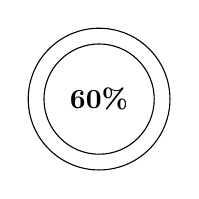
\begin{tikzpicture}
\node[draw=none]{\textbf{60\%}};
\draw (0,0) circle[radius=7mm];
\draw (0,0) circle[radius=9mm];
\centerarc[line width=0.95mm,-round cap](0,0)(90:-126:8mm)
\end{tikzpicture}}& \textbf{Barra de progreso y puntos de experiencia (XP)}

En el diseño de estrategias gamificadas, las barra de progreso se usan a menudo para reflejar el estado de los
estudiantes en el proceso de aprendizaje \cite{Li2020}. En su trabajo \citeA{DING20191} usa la barra de 
progreso para ayudar a los estudiantes a realizar un seguimiento de sus logros y como ayuda para establecer
metas, mostrando su posición frente al promedio de la clase o mostrando qué tan cerca estaban de lograr la 
siguiente meta, notando sentimientos positivos en el uso de barras de progreso al mostrar la acumulación de 
experiencia.

Por lo que las barras de progreso brindan información valiosa sobre el progreso mientras avanzan en sus
actividades, esto es útil ya que a los estudiantes no les gusta esperar, y el uso de este elemento acorta la 
percepción del tiempo y puede mejorar su tolerancia a la espera, lo que es esencial en el proceso
pedagógico.
\\
\adjincludegraphics[width=0.5\linewidth,valign=t]{mecanicas/commerce} & \textbf{Intercambio y comercio}

Son las mecánicas establecidas para que se cree un sistema de comercio o intercambio de bienes virtuales por
parte de los jugadores, promoviendo las competencias necesarias para el comercio, las motivaciones para 
conseguir bienes, y la cooperación entre jugadores.
\\
\adjincludegraphics[width=0.5\linewidth,valign=t]{mecanicas/loteria} & \textbf{Lotería (Aleatoriedad)}

Son elementos aleatorios en forma de cajas de regalos o eventos que mediante el uso del azar generan en los
jugadores sentimientos de emoción o incertidumbre, por ejemplo al no saber que objeto le va a salir, si un
evento se encuentra disponible o si un ataque será efectivo.
\\
\adjincludegraphics[width=0.5\linewidth,valign=t]{mecanicas/acknowledgment} & \textbf{Exaltaciones o correcciones: retroalimentación rápida}

Son reconocimientos positivos o negativos, que se le dan a un estudiante al momento de ejecutar una acción en
el juego, estas retroalimentaciones son puntuales al ejecutar bien o mal una actividad y no necesariamente
conlleva una recompensa, por ejemplo, un mensaje de felicitaciones al realizar bien una acción, o en caso 
contrario un mensaje indicando que algo se esta haciendo mal, por lo que estas retroalimentaciones al ser en
tiempo real al ejecutar la tarea, promueven y refuerzan la buena o mejor manera de realizarla.

Estas mecánicas de retroalimentación guían a los estudiantes y su evolución hacia el cumplimiento del objetivo
planificado en la gamificación, por lo tanto, esta retroalimentación debe ser fácilmente visible para que el 
estudiante pueda mejorar el dominio deseado. Está debe ser inmediata o en ciclos cortos, funcionando como un 
sistema de recompensa cercano al momento en que el estudiante expresan el comportamiento, en lugar
de distante y a largo plazo, estimulando así el pensamiento estratégico al ser corregido o exaltado
constantemente, lo que permite más oportunidades para obtener resultados exitosos \cite{CECHELLA2018}.
\\
\adjincludegraphics[width=0.7\linewidth,valign=t]{mecanicas/easteregg} & \textbf{Trucos y huevos de pascua}

Los huevos de pascua, son elementos ocultos pero intencionales que han dejado los desarrolladores
de un juego, con el fin de hacer referencias escondidas o atajos, lo que enriquecen aun mas la historia de un
juego, brindando elementos diegéticos adicionales, y permitiendo la rejugabilidad solamente para encontrarlos
o verlos en acción.
\\
\adjincludegraphics[width=0.6\linewidth,valign=t]{mecanicas/performance} & \textbf{Gráficos de rendimiento: retroalimentación lenta}

Los gráficos de rendimiento se utilizan a menudo en juegos de simulación o estrategia, proporcionando
información sobre el rendimiento de los estudiantes en comparación con su rendimiento anterior durante una
actividad. Por lo tanto, a diferencia de las tablas de clasificación, los gráficos de rendimiento no comparan
el  rendimiento del jugador con el de otros jugadores, sino que evalúan el propio rendimiento del jugador a lo 
largo del tiempo \cite{SAILER2017371}.
\\
\adjincludegraphics[width=0.6\linewidth,valign=t]{mecanicas/padlock} & \textbf{Elementos desboqueables}

Son elementos del juego (personajes, habilidades, misiones, equipo,  etc.) que a manera de recompensa se
habilitan (desbloquean) para que los estudiantes hagan uso de ellos dada una condición cumplida, por ejemplo,
una fecha particular, dada una acción del usuario, al subir el nivel o incluso comprarlo. La ventaja de usar
este tipo de elementos, es que puede dar pie a que el estudiante se enfoque y planee su consecución, adicional
de motivar la rejugabilidad del juego en si.
\\
\adjincludegraphics[width=0.5\linewidth,valign=t]{mecanicas/party} & \textbf{Compañeros de equipo}

La conformación de equipos ya sea con otros jugadores reales o personajes virtuales (NPCs), puede provocar
sentimientos de conflictos, competencia o cooperación según como se maneje esta mecánica \cite{SAILER2017371}.
Sin embargo, la conformación de equipos fortalece las competencias de planeación, ya que se hacen uso de las
diversas habilidades e historias que acompañan a cada personaje, creando vínculos entre estudiantes y
fortaleciendo la identidad del estudiante.
\\
\adjincludegraphics[width=0.6\linewidth,valign=t]{mecanicas/enemy} & \textbf{Obstáculos/enemigos/jefes}

En los video juegos el objetivo principal requiere habitualmente que el jugador haga uso de sus habilidades,
a menudo en un contexto de batalla o para superar obstáculos, con el fin de lograr su meta, por lo que crear
obstáculos, acertijos, jefes que motiven a la persona a superarlos es la escencia para que el juego sea
desafiante y divertido. Según \citeA{Algavi2017}, la pelea con un enemigo es un componente del juego que se 
encuentra en la base de la pirámide junto con el registro de logros, niveles, puntos, insignias, obsequios y 
otros elementos de motivación para los jugadores, por lo que se pueden diseñar una clase basada en la pelea de 
con enemigos, y entonces podría convertirse no solo en un componente de la gamificación, sino en la base para 
crear una narrativa como una forma de organizar la experiencia de los estudiantes en el marco educativo.
\\
\adjincludegraphics[width=0.5\linewidth,valign=t]{mecanicas/dummy} & \textbf{Misión de Entrenamiento}

Es una técnica usada regularmente en casi todos los videojuegos, donde se diseña una misión inicial de 
dificultad fácil para que el jugador conozca y se familiarice con las mecánicas, controles y reglas del juego. 
Por otro lado lograr captar al jugador motivándolo a seguir jugando las misiones mas difíciles.
\\
\end{longtable}
\egroup

\subsubsection{Dinámicas}

Los juegos presentan características que los hacen desafiantes, divertidos, gratificantes o con la posibilidad 
de inspirar cualquier emoción en los estudiantes. Son estas emociones el resultado de sus propios deseos y 
motivaciones lo que se denomina dinámicas de un juego, por lo que las dinámicas son todas las interacciones 
que los jugadores tienen con la mecánica establecida. En otras palabras, Las personas están motivadas por el 
juego debido a como la dinámica que este genera influye en las necesidades y deseos fundamentales que tienen 
las personas hacia el alcance de sus propios objetivos \cite{DAROCHASEIXAS201648}. A continuación se hace un 
repaso de las dinámicas mas concurrentes que se encuentran en la bibliografía sobre gamificación:

\begin{description}
\item[\textbf{Valoración}] \hfill \\ Es la sensación de ser valorado por medio de las recompensas cuando estas
se presentan después de un comportamiento por parte del estudiante, permitiendo que este comportamiento se 
repita al ser valorado \cite{DAROCHASEIXAS201648}
\item[\textbf{Reconocimiento}] \hfill \\ Representa la necesidad que tienen los estudiantes de ser
reconocidos: fama, prestigio, atención y, por último, estima y respeto de los demás, debido a sus acciones
\cite{DAROCHASEIXAS201648}.
\item[\textbf{Realización}] \hfill \\ La metas en los estudiantes puede ser nivel personal o a nivel de grupo
\cite{doi:10.1089/cyber.2012.0492}. Por lo que los estudiantes se sienten impulsados por la necesidad de
lograr algo mediante esfuerzos propios prolongados y repetidos. Las personas tienden a buscar la culminación
de desafíos y su mayor recompensa es su respectiva finalización \cite{DAROCHASEIXAS201648}.
\item[\textbf{Individualización}] \hfill \\ Los estudiantes requieren oportunidades para poder expresar su
autonomía y originalidad y, de alguna manera, diferenciarse de los demás para tener la posibilidad de crear o
mostrar su propia identidad \cite{DAROCHASEIXAS201648}. Refiriéndose al deseo intrínseco en las personas de
poder expresar su autonomía y originalidad, lo que da forma a sus personalidades únicas 
\cite{doi:10.1089/cyber.2012.0492}.
\item[\textbf{Competición}] \hfill \\ Se refiere al deseo del estudiante de tener la posibilidad de competir
con otros o contra el mismo juego bajo unas reglas, obteniendo la sensación de ganar, perder o solo competir
\cite{doi:10.1089/cyber.2012.0492}. Esto ocurre porque hay una especie de satisfacción al comparar tu propio
desempeño con el de los demás \cite{DAROCHASEIXAS201648}.

Existen dos tipos de competencia: La destructiva que ocurre cuando los estudiantes se sienten presionados o
controlados por hacia la competencia, mientras que la constructiva ocurre cuando la experiencia es placentera
\cite{DING20191}.
\item[\textbf{Altruismo}] \hfill \\ Es el deseo de las personas de tender puentes y mantener la relación con
otros mediante la realización de ciertos comportamientos, como dar regalos o pedir ayuda
\cite{doi:10.1089/cyber.2012.0492}.
\item[\textbf{Socialización}] \hfill \\ La identificación de grupo representa la lealtad afectiva y cognitiva
de los estudiantes hacia el grupo de personas que participan en un grupo de trabajo
\cite{doi:10.1089/cyber.2012.0492}.

Un aspecto importante es establecer una comunidad en la que los estudiantes se sientan conectados, y puedan
compartir valores y disfruten de una identidad compartida, apoyándose mutuamente en el esfuerzo de
aprendizaje, fomentando un sentido de grupo \cite{DING20191}. Los juegos pueden promover esta colaboración,
fomentando que los jugadores compartan conocimientos y habilidades para tener éxito en las asignaciones,
promoviendo y recompensando el trabajo en equipo tiene un impacto positivo en el desarrollo de estas dinámicas
\cite{8190501}.
\item[\textbf{Exploración y descubrimiento}] \hfill \\ A medida que los estudiantes ingresan al juego y van
desarrollándolo, se generan sentimientos en el momento de aprendizaje o descubrimiento de las mecánicas,
ambientes e historias que involucra el juego mismo \cite{doi:10.1089/cyber.2012.0492}.
\end{description}

A continuación se listan con una breve descripción otras dinámicas descritas por \citeA{Kim2018},

\begin{itemize}
\item \textbf{Cautivación:} Experiencia de olvidar el entorno donde se encuentra.
\item \textbf{Desafío:} Experiencia de tener que desarrollar o ejercitar habilidades en una situación
desafiante.
\item \textbf{Control:} Experiencia de tener poder, dominio, control o virtuosismo.
\item \textbf{Erotismo:} Experiencia por placer o excitación sexual.
\item \textbf{Expresión:} Experiencia de crear algo o expresarse de forma creativa.
\item \textbf{Fantasía:} Experiencia de fantasía que involucra narrativas, mundos o personajes fantásticos.
\item \textbf{Relajación:} Experiencia de relajación o alivio del estrés, calma durante el juego.
\item \textbf{Sadismo:} Experiencia de destrucción y ejercicio de poder sobre los demás.
\item \textbf{Sensación:} Experiencia sensorial significativa, por sonidos o imágenes.
\item \textbf{Simulación:} Experiencia de percibir una representación de la vida cotidiana.
\item \textbf{Subversión:} Experiencia de romper roles, reglas y normas sociales.
\item \textbf{Sufrimiento:} Experiencia de frustración, enojo, aburrimiento y decepción típica de jugar.
\item \textbf{Simpatía:} Experiencia de compartir sentimientos emocionales.
\item \textbf{Emoción:} Experiencia de emoción derivada de un peligro o riesgo real o percibido.
\end{itemize}

\subsubsection{Emociones}

El interés por la gamificación surge de la idea de que influye en el comportamiento de los estudiantes, 
afectando directamente sus emociones y provocando poderosas respuestas emocionales, como la curiosidad,
frustración y alegría \cite{Buckley20161162}, por lo que desde este punto de vista el aprendizaje es impulsado
por algo llamado motivación intrínseca en lugar de extrínseca \cite{Danka2020}, donde el impacto de las
intervenciones gamificadas en los estudiantes varía dependiendo de si el estudiante está motivado intrínseca o
extrínsecamente \cite{Buckley20161162}.

Aunque se reconoce ampliamente la existencia de una relación entre cognición y emoción, la ventaja de una 
sobre la otra ha sido un tema de disputas fundamentales en psicología \cite{MULLINS2020304}. Sin embargo, 
incluir elementos de juego en la educación es una forma posible de motivar a los estudiantes de manera
extrínseca hasta que estos desarrollen un compromiso intrínseco con el aprendizaje \cite{Danka2020}.

Como se vio anteriormente en la Figura \ref{img:mecanicas}, existen tres necesidades psicológicas e 
intrínsecas básicas: la necesidad de competencia, la necesidad de autonomía y la necesidad de relaciones
humanas:

\begin{itemize}
\item La necesidad de competencia se refiere a sentimientos de eficiencia y éxito al interactuar con el
entorno.
\item La necesidad de autonomía se refiere a la libertad psicológica y a la voluntad para cumplir una
determinada tarea.
\item La necesidad de relación humana se refiere a los sentimientos de pertenencia, apego y cuidado de uno
en relación con un grupo de personas significativas. Representando el deseo básico del individuo de una
integración coherente con el entorno social.
\end{itemize}

Además del aspecto motivacional intrínseco del elemento cognitivo de los juegos, se sugiere también que los
aspectos sociales y emocionales de las recompensas y las consecuencias obtenidas en los entornos de juego 
contribuyen a la motivación del estudiante \cite{8190501}.

Las experiencias de los jugadores abarcan los sentimientos subjetivos que se producen al interactuar con
el juego, mientras que los diseñadores de sistemas gamificados implementan mecánicas específicas para generar
ciertos tipos de dinámicas que influyan en estos sentimientos, se debe aclarar que la experiencia es personal,
y el juego es solo una mediación entre el estudiante y el aprendizaje, basados en el equilibrio de emociones
positivas y negativas \cite{PRESTOPNIK2015492}. La clave del éxito de la gamificación es encontrar un
equilibrio entre los resultados positivos y negativos para que los estudiantes sigan motivados para continuar y no
se sientan abrumados o desanimados \cite{8190501}. Los sistemas gamificados exitosos involucran a los
estudiantes al provocar sus emociones bien sea de forma positiva o negativa \cite{MULLINS2020304}.

\subsection{Narración de historias (\textit{Story telling})}

Los seres humanos almacenan, clasifican y recuperan información en forma de historias. Revivir y repetir
historias da placer a los humanos permitiendo así aprender y experimentar \cite{Brieger2013ExploringNC}. Por
lo que son fundamentales, e incluso definitorias en el aprendizaje y la cultura humanos. \citeA<En palabras de
Sartre citado por>{Young2015199} ``Un hombre es siempre un narrador de historias. Vive rodeado de sus propias
historias y las de otras personas. Ve todo lo que le pasa en términos de estas historias y trata de vivir su
vida como si la estuviera contando'', es por eso que se puede concluir que los humanos evolucionaron para 
entender sus vidas en términos del uso de estructuras narrativas, en este contexto darwiniano, la narrativa
eficaz se adaptó a nuestra especie y fuimos seleccionados para aprender a través de las historias
\cite{Young2015199}.

Es a través de la narrativa que se comparten conocimientos, se fomenta la indagación y se promueven la 
creatividad \cite{Young2015199}. En particular para los juegos basados en historias estos pueden ser más
útiles para atraer e involucrar a los estudiantes desmotivados en la participación de los procesos pedagógicos
\cite{PRESTOPNIK2015492}. Los juegos basados en narración de historias para el desarrollo de procesos 
educativos pueden dar la libertad de adoptar una pedagogía creativa, acomodando una amplia variedad de 
discapacidades, antecedentes e intereses de los estudiantes.

Es por esto, que el modelo de narración de historias en educación presenta grandes ventajas para que los 
estudiantes se sientan identificados con aspectos que acontecen en la historia. Es esa empatía la que permite 
que se creen sus propios juicios y opiniones sobre el proceso educativo que están vivenciando a través de la
narración \cite{tornero2016ideas}.

Actualmente, existe la oportunidad de crear historias flexibles, creadas en forma de una narrativa no lineal, 
donde estas no trascurren de principio a fin de forma tradicional; en cambio, le dan al estudiante la opción
de seguir diferentes caminos. Promoviendo en los estudiantes un sentido de autonomía y responsabilidad 
personal sobre su proceso de aprendizaje logrado a través de esta narración no lineal, ya que las elecciones
que hace el estudiante en la historia cambian el resultado final, ofreciendo la capacidad de aprender de sus
errores en un entorno seguro y sin riesgos \cite{trevor2017}.

Al igual que las formas más tradicionales de narrativa, los videojuegos no son estáticos, sino que se
presentan en contexto, son emergentes, sobre la marcha e interactivamente con el contexto dinámico establecido
por múltiples jugadores simultáneos. \cite{Young2015199} Es por eso, que se puede decir existen dos tipos de
narrativa que se ocupan de la experiencia del jugador: incrustada y emergente \cite{SBIE8805}, donde la
incrustada es la que se encuentra como base en la historia del juego, y la emergente es aquella que se forma
gracias a la experiencia de los estudiantes interactuando con los elementos del juego.

La narrativa en los videojuegos se puede discriminar por lo tanto en tres niveles de profundidad
\cite{Young2015199}:

\begin{description}
\item[Nivel 1] \hfill \\ Narrativa del vídeo juego (Incrustada)
\item[Nivel 2] \hfill \\ Narrativa creada por las acciones de los jugadores (Emergente)
\item[Nivel 3] \hfill \\ Narrativa creada a partir de la interacción social entre los jugadores, se produce
fuera del ámbito del propio juego.
\end{description}

Tiene poco sentido asumir que las historias se interpretan exactamente como se pensaron en la cabeza del 
narrador, es por esto que las experiencias individuales del estudiante (lector) varía de acuerdo a su
contexto, su percepción e intencionalidad. Es por esto que el contenido y el entorno de la narración, pueden
conducir hacia el descubrimiento de nuevos y diferentes posibilidades ofrecidas por las elementos de la
historia, personajes y escenarios \cite{Young2015199}.

\subsection{Juegos de Rol (\textit{Role-Playing Gaming, RPG)}}

Los juegos de rol son un género en el que los jugadores controlan un solo personaje (que tiene habilidades 
específicas, personalidad, estilo de combate, etc.) y deben convertirse en uno con él, y actuando como si 
fueran esa persona a través del entorno del juego. Esta idea se origina en los juegos de rol de mesa, como 
\textit{Dungeons and Dragons}, también conocido como D\&D \cite{Ntokos2019, gygax1979dungeons}.

Los juegos de rol (RPG) utilizan una combinación de rasgos del personaje, puntos de experiencia y nivelación
para ilustrar cómo un personaje evoluciona y se fortalece a medida que avanza en el juego \cite{Li2020}. Al
proporcionar conexiones sólidas entre el comportamiento y las elecciones del estudiante, en el desarrollo de
su personaje, los juegos de rol alientan a identificarse y crear un sentido de propiedad sobre su proceso.

Según \citeA{Li2020} indica que la gamificación puede motivar e involucrar a los estudiantes en su proceso de
aprendizaje, especialmente si se usan elementos integrados de juegos de rol (RPG). Los juegos de roles son
estrategias muy motivadoras ya que los estudiantes pueden probar diferentes roles sin demasiado compromiso. La
construcción de identidad es un factor clave en la popularidad de los juegos tipo MMORPG \cite{Danka2020}. Es
el uso de este tipo de recursos que logran convertir algo aburrido en su contraparte creativa, dando un mayor
significado a aquellos que se involucran por completo en el juego \cite{Ntokos2019}.

Por ejemplo, \textit{Dungeons \& Dragons} introdujo el concepto de fusionar un sistema de juego con un arco
narrativo inmersivo que consta de múltiples misiones o desafíos, asignando puntos y niveles de experiencia
como una forma de cuantificar el desarrollo y la progresión del personaje en múltiples episodios de juego. 
Estas y otras mecánicas RPG únicas, inicialmente apreciadas por solo una pequeña subcultura de jugadores de 
mesa, finalmente se integraron con el surgimiento de los CRPG comercialmente exitosos y, más tarde, los 
MMORPG, que también agregaron nuevas mecánicas como sistemas de logros digitales repletos de insignias y 
tablas de clasificación \cite{byers2016the, gygax1979dungeons}. Sin embargo, podemos resumir las 
características básicas de los juegos de rol en siete elementos fundamentales:

\begin{description}
\item[\textbf{Maestro del juego \textit{(Game master)}}] \hfill \\ Es la persona encargada de crear la 
narrativa y supervisar el juego de rol. Por lo que define las consecuencias de los actos de los personajes, 
describe las escenas e interpreta a los personajes NPCs que interactúan con los jugadores.

Bajo el contexto de aula, son los profesores quienes habitualmente toman este rol convirtiéndose en 
participantes activos del entorno de aprendizaje basado en roles, y sus actuaciones se extienden más allá de 
las de un docente tradicional. Actúan como agentes de control de misión, que se encargan de crear, organizar y 
dirigir el juego de roles, permitiendo dar forma al entorno de aprendizaje en tiempo real y enfatizar en las 
habilidades y los conocimientos que se consideran más importantes para la aplicación en el mundo real, 
logrando aplicar una evaluación formativa \cite{Young2015199}. 
\item[\textbf{Ficha del personaje}] \hfill \\ El primer paso para poder jugar un juego de rol es imaginar y 
crear un personaje propio. Los personajes son una combinación de estadísticas de juego y la propia imaginación
del jugador, se debe seleccionar una especie, personalidad y trasfondo, adicional se asignan unas
características (fuerza, destreza, constitución, inteligencia, sabiduría y carisma) y habilidades mágicas o
físicas, que van a ser la base de cómo el personaje creado va a sortear las dificultades y escenarios que la
aventura le plantee.
\item[\textbf{Equipamiento}] \hfill \\ En un juego de rol, el uso de armaduras, armas, mochilas, cuerdas y 
bienes similares son básicos para potenciar las habilidades del personaje, ya que el equipo adecuado puede 
significar la diferencia entre la victorea y la derrota, o sortear una dificultad en el juego.
\item[\textbf{Equipo \textit{(Party)}}] \hfill \\ Denominamos equipo o \textit{party} a la conformación de un
conjunto seleccionado de personajes, los que conforman un grupo de compañeros para sortear una aventura.
Habitualmente aunque no necesariamente cada uno con sus habilidades únicas que soportan a las de los demás
miembros del equipo.
\item[\textbf{Búsqueda \textit{(Quest)}}] \hfill \\ No importa el tipo de aventura que se esté desarrollando,
el juego sigue un ritmo natural: (1) el maestro del juego describe el entorno, (2) los jugadores describen lo
que quieren hacer y (3) el maestro del juego narra los resultados de sus acciones, y vuelve a iniciar el
ciclo. La búsqueda en si, es la razón por la que los personajes se movilizan, en este tipo de juegos las 
búsquedas pueden ser de diferentes tipos: para derrotar a un enemigo, de entrega (encontrar y entregar algún 
objeto), recolectar algún recurso, proteger un elemento del juego, o una combinación de estas.
\item[\textbf{Combate}] \hfill \\ El combate en juego de rol se desarrolla por turnos, en el desarrollo de la
aventura los personajes se enfrentarán a monstruos, trampas o acertijos, y pueden sortearlos mediante el uso
de golpes con armas, correr, esquivar, lanzamiento de conjuros, uso de objetos, ocultarse, buscar, curarse y 
ayudar.
\item[\textbf{Bitácora \textit{(Logbook)}}] \hfill \\ En los juegos de rol el maestro del juego envía a sus 
jugadores a aventuras maravillosas en las que se debe dibujar mapas para recordar el camino o ubicación de los 
personajes, y tomar registro sobre la evolución de estos, los hechizos que lanzaron y los obstáculos o 
enemigos superados. Esta bitácora es una herramienta indispensable para registrar y organizar toda la 
información que ayuda en las aventuras durante el transcurso de estas o como recuerdo una vez terminada.
\end{description}

\subsection{Teorías de aprendizaje orientadas a gamificación}

Los estudios científicos investigan cada vez más el uso de diferentes fundamentos teóricos como la motivación, 
el comportamiento o las teorías del aprendizaje para explicar el efecto de ciertos elementos de gamificación 
\cite{KRATH2021106963}. La estrategia motivacional juega un papel importante en el compromiso del estudiante 
con el aprendizaje, siendo la teoría de la autodeterminación (\textit{self-determination theory}) el eje 
central en los desarrollos gamificados, a continuación se hace una descripción de algunas de las teorías mas 
usadas según la investigación de \citeA{KRATH2021106963}:

\subsubsection{Teoría de la autodeterminación (\textit{Self-determination theory})}

La teoría de la autodeterminación expuesta por \citeA{deci1985intrinsic}, tiene como objetivo explicar la 
necesidades que conllevan la motivación humana, haciendo centro en la motivación como motor de las decisiones 
que toman las personas. Esta teoría manifiesta que el comportamiento humano es auto-motivado y
autodeterminado, y la motivación surge de tres necesidades psicológicas básicas: autonomía, competencia y 
relaciones humanas.

\begin{figure}[ht]
\caption{Necesidades psicológicas básicas, teoría de la autodeterminación}
\label{img:SDT}
\centering
\begin{tikzpicture}[
		every node/.append style={circle,draw=gray!80,align=center,minimum width=80pt,very thin}
  	]
	\node[] (A) at (-5,3.5) {
		\textbf{Autonomía}
	};
	\node[] (C) at (0,3.5) {
		\textbf{Competencia}
	};
	\node[] (R) at (5,3.5){
		\textbf{Relaciones}\\\textbf{Humanas}
	};
	\node[] (M) at (0,0){
		\textbf{Motivación}
	};
	\draw[-triangle 90,bend right] (A) edge (M);
	\draw[-triangle 90] (C) edge (M);
	\draw[-triangle 90,bend left] (R) edge (M);
\end{tikzpicture}
\\
{\footnotesize Fuente: \citeA<basada en>{deci1985intrinsic}}
\end{figure}

\subsubsection{Teoría del flujo en psicología (\textit{Flow theory})}

La teoría del flujo en psicología expuesta por \citeA{csikszentmihalyi_1988}, trata sobre el estudio del estado 
mental óptimo en el que una persona está completamente inmersa en la culminación de una actividad, bajo un
estado total de concentración y motivación hacia el proceso. Según esta teoría se puede ingresar al estado de 
``flujo'' (inmersión total) mientras se realiza cualquier actividad, aunque es más probable que ocurra este
estado cuando la tarea se realiza bajo una motivación intrínseca.

\begin{figure}[ht]
\caption{Tipo de experiencia como relación entre nivel de desafío y habilidades}
\label{img:tflow}
\centering
\begin{tikzpicture}
	\draw (0,0) -- (6,0) -- (6,6) --(0,6) -- (0,0);
	\draw[pattern=dots] (3,3) -- (4,6) -- (6,6) -- (6,4) -- (3,3);
	\draw (2,0) -- (4,6);
	\draw (4,0) -- (2,6);
	\draw (0,2) -- (6,4);
	\draw (0,4) -- (6,2);
	\node at (3,-1) {Nivel de Habilidad};
	\node at (1,-0.3) {Bajo};
	\node at (3,-0.3) {Medio};
	\node at (5,-0.3) {Alto};
	\node[rotate=90] at (-1,3) {Nivel de Desafío};
	\node[rotate=90] at (-0.3,1) {Bajo};
	\node[rotate=90] at (-0.3,3) {Medio};
	\node[rotate=90] at (-0.3,5) {Alto};
	\node at (3,0.5) {\small Tedio};
	\node at (3,5.5) {\small Exitación};
	\node at (1.25,3) {\small Preocupación};
	\node at (4.75,3) {\small Control};
	\node[rotate=45] at (5,5) {\colorbox{white}{\small Flujo}};
	\node[rotate=-45] at (5,1) {\small Relajación};
	\node[rotate=-45] at (1,5) {\small Anxiedad};
	\node[rotate=45] at (1,1) {\small Apatía};
\end{tikzpicture}
\\
{\footnotesize Fuente: \citeA<basada en>{csikszentmihalyi_1988}}
\end{figure}

\subsubsection{Teoría del establecimiento de metas (\textit{Goal-setting theory})}

La teoría del establecimiento de metas descrita por \citeA{Locke1968}, establece una explicación motivacional
del por qué algunas personas se desempeñan mejor que otras realizando una misma actividad. Se basa en la idea
que las metas específicas difíciles conducen a un rendimiento significativamente más alto que las metas 
fáciles, así como mantener un compromiso constante con el objetivo bajo limitaciones de tiempo realistas y por
último las variables como la valoración, retroalimentación o la participación en la toma de decisiones sobre 
el objetivo solo influyen en el comportamiento en la medida en que estas conduzcan al establecimiento y 
posterior compromiso con un objetivo específico difícil.

Por lo tanto, establecer metas significa que una persona ha dedicado pensamientos, emociones y acciones para 
lograr terminarla. Al hacerlo, la persona establece un estado futuro deseado que difiere de su estado actual, 
creando así un desajuste que a su vez estimula acciones futuras. Asumiendo que es la motivación y no la 
habilidad, la que limita el alcance del objetivo, existe una relación lineal positiva entre la dificultad del 
objetivo y el desempeño en la ejecución de la tarea.

\begin{figure}[ht]
\caption{Principios para un efectivo establecimiento de metas}
\label{img:goal}
\centering
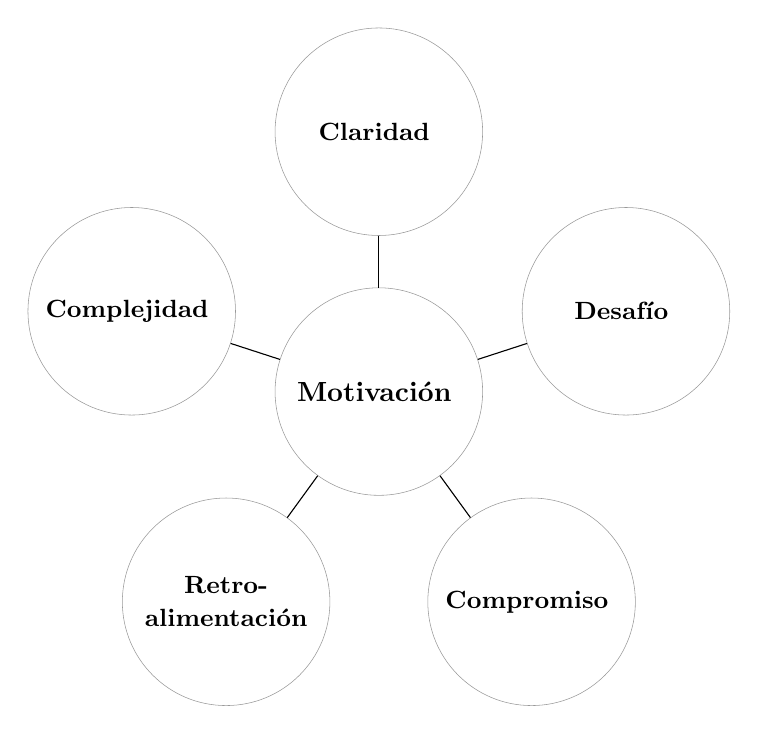
\begin{tikzpicture}[
		every node/.append style={circle,draw=gray!80,align=center,minimum width=75pt,very thin}
  	]
	\node[] (L) at (90:3.3) {
		\textbf{\small Claridad}
	};
	\node[] (D) at (18:3.3) {
		\textbf{\small Desafío}
	};
	\node[] (J) at (162:3.3){
		\textbf{\small Complejidad}
	};
	\node[] (R) at (234:3.3){
		\textbf{\small Retro-}\\\textbf{\small alimentación}
	};
	\node[] (C) at (306:3.3){
		\textbf{\small Compromiso}
	};
	\node[] (M) at (0,0){
		\textbf{Motivación}
	};
	\draw[-] (L) edge (M);
	\draw[-] (D) edge (M);
	\draw[-] (J) edge (M);
	\draw[-] (R) edge (M);
	\draw[-] (C) edge (M);
\end{tikzpicture}
\\
{\footnotesize Fuente: \citeA<basada en>{Locke1968}}
\end{figure}

Como lo muestra la Figura \ref{img:goal}, la teoría del establecimiento de metas establece cinco principios 
los cuales influencian la motivación de las personas para el logro de un objetivo:

\begin{itemize}
\item \textbf{Claridad} Los objetivos deben ser claros y bien definidos, por ejemplo siguiendo el principio 
S.M.A.R.T. (específicos, cuantificable, asignable, realista y realizable en el tiempo).
\item \textbf{Desafío} Cuando una meta es desafiante tiende a ser más motivadora y la sensación de logro 
cuando se alcanza es más significativa. Por otro lado Cuando algo es demasiado fácil, se siente menos 
importante y es más probable que pierda el enfoque y la motivación.
\item \textbf{Compromiso} Para lograr un objetivo con éxito se debe estar completamente comprometido. Es este
compromiso el que mantendrá a la persona en movimiento cuando encuentre obstáculos.
\item \textbf{Retroalimentación} La reflexión constante del proceso para alcanzar un objetivo ayuda a 
mantener a las personas encaminadas y motivadas, al garantizar que sus objetivos siguen siendo relevantes.
\item \textbf{Complejidad} El rendimiento de la tarea se puede optimizar considerando primero su complejidad
al establecer una línea de tiempo para cumplirla. Por lo que se debe asegurar las condiciones para no frustrar
ni impedir se logren reforzando la posibilidad de lograrlas.
\end{itemize}

\subsubsection{Teoría cognitiva social (\textit{Social cognitive theory})}

La teoría cognitiva social fue planteada por \citeA{bandura1986social}, como una extensión de la teoría de 
aprendizaje social, esta teoría postula que el aprendizaje se forma a través de la interacción de tres
factores: sociales, cognitivos y de comportamiento. Los factores sociales se refieren a aquellos que se 
aprenden mediante la observación, los factores cognitivos se derivan de interpretaciones cognitivas del 
entorno social observado y el comportamiento deseado que se manifiesta como una consecuencia por los dos 
factores anteriores.

\begin{figure}[ht]
\caption{Teoría cognitiva social}
\label{img:TCS}
\centering
\begin{tikzpicture}[
		every node/.append style={draw=none,align=center}
  	]
	\node[] (S) at (170:3) {\textbf{Social}\\\textbf{\small Factores ambientales}};
	\node[] (C) at (10:3) {\textbf{Cognitivo}\\\textbf{\small Factores personales}};
	\node[] (M) at (270:2) {\textbf{Comportamiento}\\\textbf{\small Aprendizaje, motivación}};
	\draw[{Stealth[length=3mm,width=2mm]}-{Stealth[length=3mm,width=2mm]}] (S) edge (C);
	\draw[{Stealth[length=3mm,width=2mm]}-{Stealth[length=3mm,width=2mm]}] (C) edge (M);
	\draw[{Stealth[length=3mm,width=2mm]}-{Stealth[length=3mm,width=2mm]}] (M) edge (S);
\end{tikzpicture}
\\
{\footnotesize Fuente: \citeA<basada en>{bandura1986social}}
\end{figure}

\subsubsection{Teoría del reforzamiento conductual (\textit{Behavior reinforcement theory})}

La teoría del reforzamiento conductual propuesta por \citeA{skinner1969contingencies}, afirma que el 
comportamiento de una persona se manifiesta en función de las consecuencias de sus actos, es decir, el 
comportamiento que tiene consecuencias positivas tiende a repetirse, pero el comportamiento con consecuencias
negativas tiende a no repetirse, esta teoría ignora los sentimientos internos de los individuos centrándose 
totalmente en lo que le sucede cuando este realiza alguna acción y no lo que siente.

\begin{figure}[ht]
\caption{Teoría del reforzamiento conductual}
\label{img:TRC}
\centering
\begin{tikzpicture}
\node[draw,regular polygon, regular polygon sides=4,minimum width=120pt,align=center,draw=gray!80] (RP) at (-90pt,0) {\textbf{Refuerzo}\\\textbf{positivo}};
\node[draw,regular polygon, regular polygon sides=4,minimum width=120pt,align=center,draw=gray!80] (RN) at (0,0) {\textbf{Refuerzo}\\\textbf{negativo}};
\node[draw,regular polygon, regular polygon sides=4,minimum width=120pt,align=center,draw=gray!80] (CP) at (-90pt,-90pt) {\textbf{Castigo}\\\textbf{positivo}};
\node[draw,regular polygon, regular polygon sides=4,minimum width=120pt,align=center,draw=gray!80] (CN) at (0,-90pt) {\textbf{Castigo}\\\textbf{negativo}};
\node[draw=none] at (-90pt,60pt) {$+$Estimulo};
\node[draw=none] at (0pt,60pt) {$-$Estimulo};
\node[draw=none,rotate=90] at (-150pt,0pt) {$+$Conducta};
\node[draw=none,rotate=90] at (-150pt,-90pt) {$-$Conducta};
\end{tikzpicture}
\\
{\footnotesize Fuente: \citeA<basada en>{skinner1969contingencies}}
\end{figure}

Como se puede ver en la Figura \ref{img:TRC} esta teoría hace uso de cuatro mecanismos para controlar el
comportamiento de las personal:

\begin{itemize}
\item \textbf{Refuerzo positivo:} Emitir un estímulo para aumentar la probabilidad de una conducta. Por 
ejemplo, dar un premio al hacer una actividad.
\item \textbf{Refuerzo negativo:} Retirar un estímulo negativo para aumentar la probabilidad de una conducta.
Por ejemplo, quitar un castigo al hacer una actividad.
\item \textbf{Castigo positivo:} Emitir un estímulo para disminuir la probabilidad de una conducta. Por 
ejemplo, dar un castigo por no hacer la actividad.
\item \textbf{Castigo negativo:} Retirar un estímulo para disminuir la probabilidad de una conducta. Por 
ejemplo, quitar privilegios por no hacer una la actividad.
\end{itemize}

\subsubsection{Teoría de la identidad social (\textit{Identity theory})}

La teoría de la identidad social expuesta por \citeA{tajfel1979integrative}, tiene como objetivo especificar y
predecir las circunstancias bajo las cuales las personas se consideran a sí mismos como individuos o como 
miembros de un grupo, considerando las consecuencias de las identidades personales y sociales para las 
percepciones individuales y el comportamiento grupal.

\begin{itemize}
\item \textbf{Categorización social:} Las personas categorizan a otras para identificarlas y comprenderlas.
\item \textbf{Identificación social:} Las personas adoptan la identidad del grupo en el que se clasifican.
\item \textbf{Comparación social:} Las personas tienden a comparar el grupo al que pertenecen con otros
grupos.
\end{itemize}

\begin{figure}[ht]
\caption{Teoría de la identidad social}
\label{img:TIS}
\centering
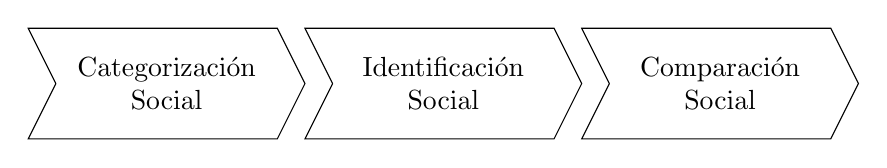
\begin{tikzpicture}
\node[draw=none,align=center] at (-100pt,0pt) {Categorización\\Social};
\node[draw=none,align=center] at (0pt,0pt) {Identificación\\Social};
\node[draw=none,align=center] at (100pt,0pt) {Comparación\\Social};
\draw (-140pt,0pt) -- (-150pt,20pt) -- (-60pt,20pt) -- (-50pt,0pt) -- (-60pt,-20pt) -- (-150pt,-20pt) -- (-140pt,0pt);
\draw (-40pt,0pt) -- (-50pt,20pt) -- (40pt,20pt) -- (50pt,0pt) -- (40pt,-20pt) -- (-50pt,-20pt) -- (-40pt,0pt);
\draw (60pt,0pt) -- (50pt,20pt) -- (140pt,20pt) -- (150pt,0pt) -- (140pt,-20pt) -- (50pt,-20pt) -- (60pt,0pt);
\end{tikzpicture}
\\
{\footnotesize \citeA<basada en>{tajfel1979integrative}}
\end{figure}

\subsubsection{Modelo ARCS (\textit{ARCS model})}

Este modelo fue descrito por \citeA{keller1983motivational}, su base radica en el estudio de cuatro elementos 
claves que permiten estimular y mantener la motivación durante el proceso de aprendizaje, las cuatro 
categorías forman el acrónimo ARCS: Atención, Relevancia, Confianza y Satisfacción, 

\begin{itemize}
\item \textbf{Atención:} Antes que el proceso de aprendizaje inicie se requiere tener la atención de los 
estudiantes, por lo que esta relacionada con conseguir y mantener el interés de los alumnos, para que estos 
estén enfocados y comprometidos con la temática de estudio,
\item \textbf{Relevancia:} Se refiere a hacer que la experiencia de aprendizaje sea relevante o significativa 
para el estudiante.
\item \textbf{Confianza:} Lograr en los estudiantes auto-eficacia y una expectativa de éxito respecto a su 
proceso de aprendizaje, generando sentimientos positivos al poder conseguir los objetivos.
\item \textbf{Satisfacción:} Es el desarrollo del deseo persistente por aprender, debido al sentimiento de 
satisfacción del estudiante por lograrlo, mediante recompensas y refuerzos que medien en la motivación 
intrínseca o extrínseca.
\end{itemize}

%\subsubsection{Teoría de la actividad (\textit{Activity theory})}
%\subsubsection{Modelo ARCS (\textit{Eisenkraft's 7E Instructional Model })}
%\subsubsection{Modelo ARCS (\textit{attribution theory})}
%\subsubsection{Modelo ARCS (\textit{mood management theory})}
%\subsubsection{Modelo ARCS (\textit{situated learning theory})}

